%! Author = lili
%! Date = 8/12/26

\section{Abgabe 2.2}\label{sec:abgabe-2.2}

\subsection{HA 2.2.1 (teils)}\label{subsec:ha-2.2.1}
Betrachten Sie folgendes Spiel mit zwei fairen Würfeln: Wenn der Spieler einen Pasch wirft (beide Würfel zeigen die gleiche Augenzahl), so sei die Auszahlung die Augensumme in Euro.
Andernfalls erhält der Spieler keine Auszahlung.

\textit{Denken Sie daran, einen Wahrscheinlichkeitsraum anzugeben und die benötigten Zufallsvariablen zu definieren!}

\begin{auf}[(a) Wie muss der Einsatz für das Spiel gewählt werden, damit das Spiel fair ist?]
    NOCH KEINE LÖSUNG % TODO NOCH KEINE LÖSUNG
\end{auf}

\begin{auf}[(b) Es werden 200 Runden gespielt, und der Betreiber möchte einen erwarteten Gewinn von 100 Euro erzielen. Wie hoch muss nun der Einsatz pro Runde gewählt werden?]
    NOCH KEINE LÖSUNG % TODO NOCH KEINE LÖSUNG
\end{auf}

\begin{auf}[(c) Geben Sie mit Hilfe der Tschebyscheff-Ungleichung eine untere Schranke an für die Wahrscheinlichkeit, dass der Betreiber bei 200 Runden wenigstens keinen Verlust erleidet, wenn er den in (b) berechneten Spieleinsatz pro Runde erhebt.]
    $\ $
    \begin{figure}[H]
        \centering
        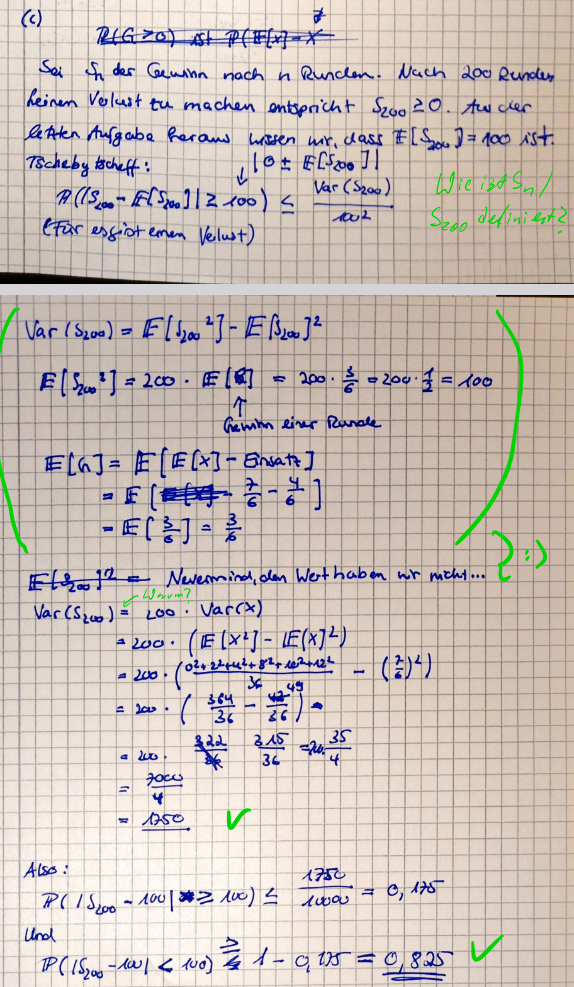
\includegraphics[width=0.8\linewidth]{images/lösungen/wts221c}\label{fig:figure55}
    \end{figure}
\end{auf}

\begin{auf}[(d) Schätzen Sie mit Hilfe der Tschebyscheff-Ungleichung ab, wie viele Runden mit dem in (b) bestimmten Spieleinsatz pro Runde mindestens gespielt werden müssen, damit der Betreiber mit einer Wahrscheinlichkeit von mindestens 90\% wenigstens keinen Verlust erleidet.]
    $\ $
    \begin{figure}[H]
        \centering
        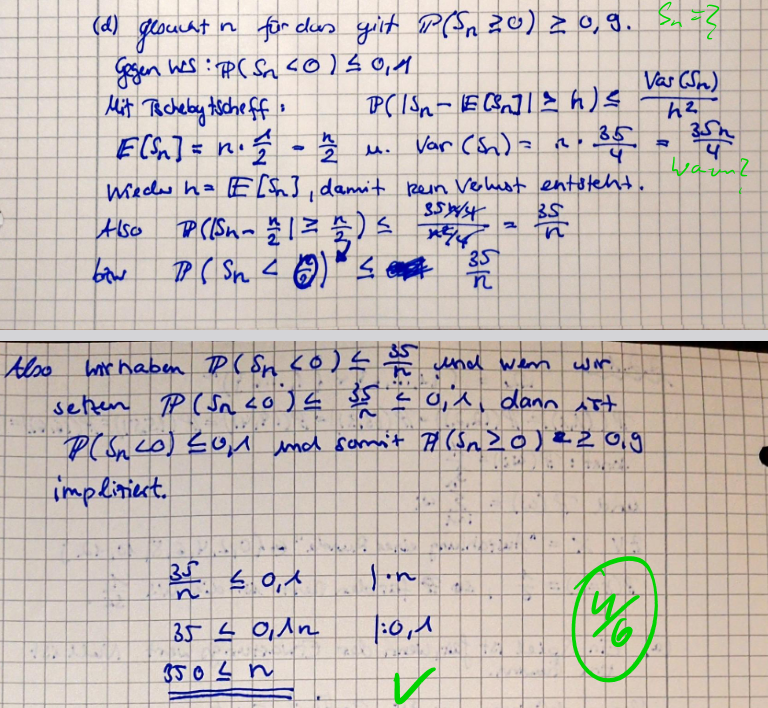
\includegraphics[width=0.8\linewidth]{images/lösungen/wts221d}\label{fig:figure54}
    \end{figure}
\end{auf}

\subsection{HA 2.2.2 (nicht vorhanden)}\label{subsec:ha-2.2.2}

\subsection{HA 2.2.3 (teils)}\label{subsec:ha-2.2.3}
Eine Firma produziert Gummibärchen in fünf verschiedenen Farben.
Eine Studie aus der Marktforschung hat ergeben, dass Rot die beliebteste Farbe für Gummibärchen ist.
Daher ist $\frac13$ der hergestellten Gummibärchen rot.
Die Abfüllung ist so eingestellt, dass die Gummibärchen zufällig in Tüten von 162 Stück abgefüllt werden.
Wir haben eine dieser Tüten gekauft.

\begin{auf}[(a)  Geben Sie einen geeigneten Wahrscheinlichkeitsraum an, der es erlaubt, die folgenden Aufgabenteile zu bearbeiten. Diskutieren Sie, welche Annahmen Sie machen müssen, um Ihre Wahl des Wahrscheinlichkeitsraums zu rechtfertigen.]
    $\ $
    \begin{figure}[H]
        \centering
        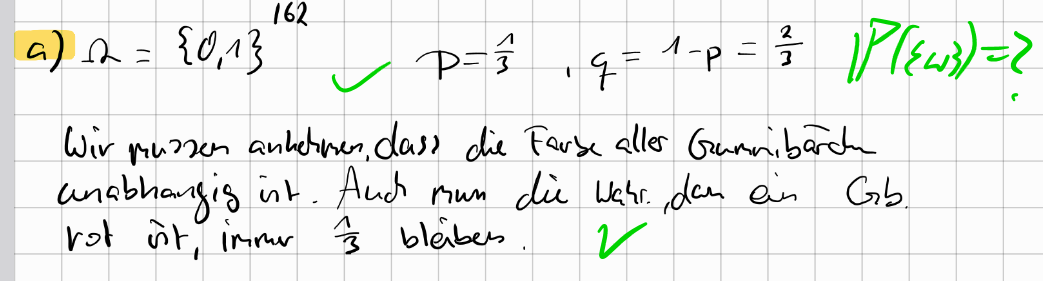
\includegraphics[width=0.8\linewidth]{images/lösungen/wts223a}\label{fig:figure53}
    \end{figure}
\end{auf}

\begin{auf}[(b) Definieren Sie eine Zufallsvariable $S_{162}$, die angibt, wie viele rote Gummibärchen in der Tüte sind. Welcher Verteilung folgt die Zufallsvariable $S_{162}$? Geben Sie gegebenenfalls die zugehörigen Parameter an.]
    $\ $
    \begin{figure}[H]
        \centering
        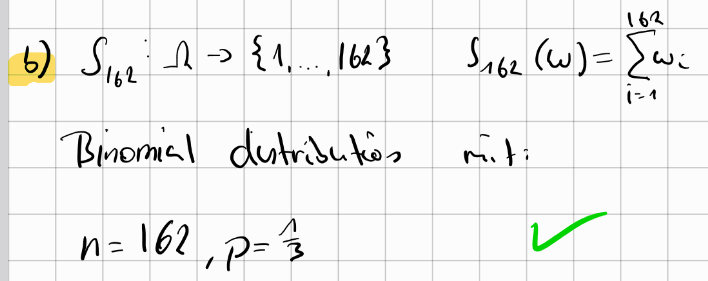
\includegraphics[width=0.8\linewidth]{images/lösungen/wts223b}\label{fig:figure52}
    \end{figure}
\end{auf}

\begin{auf}[(c) Bestimmen Sie Erwartungswert und Varianz von $S_{162}$.]
    $\ $
    \begin{figure}[H]
        \centering
        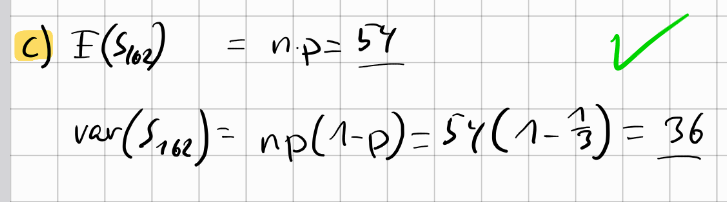
\includegraphics[width=0.8\linewidth]{images/lösungen/wts223c}\label{fig:figure51}
    \end{figure}
\end{auf}

\begin{auf}[(d) Bestimmen Sie näherungsweise unter Verwendung des Satzes von de Moivre--Laplace (mit und ohne Stetigkeitskorrektur) die Wahrscheinlichkeit, dass zwischen (einschließlich) 40 und (einschließlich) 69 rote Gummibärchen in der Tüte enthalten sind. Bestimmen Sie auch das exakte Ergebnis.]
    NOCH KEINE LÖSUNG % TODO NOCH KEINE LÖSUNG
\end{auf}

\begin{auf}[(e) Bestimmen Sie näherungsweise unter Verwendung des Satzes von de Moivre--Laplace (mit und ohne Stetigkeitskorrektur) auch die Wahrscheinlichkeit, dass zwischen (einschließlich) 43 und (einschließlich) 60 rote Gummibärchen in der Tüte enthalten sind. Bestimmen Sie auch das exakte Ergebnis.]
    NOCH KEINE LÖSUNG % TODO NOCH KEINE LÖSUNG
\end{auf}

\begin{auf}[Was fällt Ihnen auf, wenn Sie die Ergebnisse aus (d) und (e) miteinander vergleichen?]
    NOCH KEINE LÖSUNG % TODO NOCH KEINE LÖSUNG
\end{auf}

